\documentclass[driverfallback=dvipdfmx,cjk]{beamer}

\usepackage{bxdpx-beamer}% dvipdfmxなので必要
\usepackage{pxjahyper}% 日本語で'しおり'したい
\usepackage{minijs}% min10ヤダ
\renewcommand{\kanjifamilydefault}{\gtdefault}% 既定をゴシック体に

\AtBeginShipoutFirst{\special{pdf:tounicode 90ms-RKSJ-UCS2}}
%\AtBeginSection[]{
%    \frame{\tableofcontents[currentsection, hideallsubsections]} %目次スライド
%}
%\usepackage{amsmath,amssymb}
\usetheme{Antibes}
\usefonttheme{professionalfonts}
\usepackage{color}
\usepackage{mediabb}
\usepackage[absolute,overlay]{textpos}
%\usetheme{Madrid}
%
%\usecolortheme{albatross}
\useinnertheme{circles}
\setbeamertemplate{navigation symbols}{}
\setbeamertemplate{footline}[page number]
\setcounter{tocdepth}{2}


\title{XVA and its Greeks Calculation}
\author{森本 裕介}
\institute{三菱UFJ銀行}
\date{2018/11/23 - 11/25 \\ 第6回 数理ファイナンス合宿型セミナー}

%%%%%% TEXT START %%%%%%
\begin{document}
\begin{frame}
\titlepage
本講演の内容は発表者個人に属し所属する組織の公式見解を示すものではない。
\end{frame}


\begin{frame}\frametitle{Contents}
    \begin{itemize}
        \item Definition of XVA
        \begin{itemize}
            \item Introduction
            \item Semi-Replication
        \end{itemize}
        \item Calculation of XVA
        \begin{itemize}
           \item XVAの計算法
           \item Implicit法 
        \end{itemize}
        \item Greeks calculation of XVA
        \begin{itemize}
           \item XVA Greeksの計算法
           \item Freezing法
           \item Automatic Differentiation (AD)
        \end{itemize}
    \end{itemize}
\end{frame}

\begin{frame}
    \textbf{Definition of XVA}
\end{frame}

\section{Definition of XVA}
\subsection{Introduction}
\begin{frame} 
    \begin{itemize}
        \item $V$ : 従来のデリバティブの価値
            \begin{itemize}
                \item Counter party default risk を考慮しない
                \item 自社の default risk を考慮しない
                \item 自社のFunding コストを考慮しない
                \item 担保のcash flowを考慮しない(考慮したとしても完全担保 )
            \end{itemize}
        \item $\hat{V}$ : 上記に付随する金利のスプレッドやCash flowを考慮したデリバティブの価値
    \end{itemize}
    $$\hat{V} = V + U, $$
    $$U = \sum_{X=C, D, F, M, ...} \textcolor{red}{X}VA$$
    \begin{itemize}
        \item CVA: counterparty credit risk adjustment
        \item DVA: Own credit risk adjustment
        \item FVA: Funding cost
        \item MVA: Margin cost
    \end{itemize}
\end{frame}

\begin{frame}
    \begin{itemize}
        \item $\hat{V}, U$ の導出
        \begin{itemize}
            \item Piterburg(2010):
            Replication theory を使ったFVAの導出
            \item Burgard and Kjaer(2011,  2013), Kjaer(2017):
            Semi-ReplicationによるXVAの定式化(Quant of the year)
            \item Green, Knyon():
            Semi-Replicationに基づくKVA, MVA 等の導入
            \item その他の定式化 : Fuji and Takahashi(2014), Kusuoka(2013), Takada(2014)
        \end{itemize}
        \item XVA(FVA)の定義をめぐる議論
        \begin{itemize}
            \item Hull-White(2012, 2013)
            \begin{itemize}
                \item PricingはFundingと切り離して行われるべき
                \item Modiliani-Millarの定理: 企業価値はFunding strategyに依存しない 
            \end{itemize}
            
            \item Albanese and Andersen(2015)\\
            バランスシートを使った議論、株主価値と企業価値の導入
            \item Kjaer(2017) \\
            Semi Replicationを使った株主価値と企業価値の解釈
        \end{itemize}
    \end{itemize}
\end{frame}

\subsection{Semi Replication}
\begin{frame} 
    \textbf{Semi Replication}\\
    Semi-Replicationの概要(Burgard-Kjaer 2013, Kjaer 2017)
    \begin{itemize}
        \item Setting
        \begin{itemize}
            \item $X$ : spot asset price \ 
            $ dX = \mu^X Xdt + \sigma^X X dW_X ,$
            \item $P^B, P^C$: bank and counterparty \textcolor{red}{defaultable} bond 
            $$dP^* = r^* P^*(t-) dt - (1-R^*) P^*(t-) dJ^*, *=B,C$$
            \item $\beta^{*}$ : asset and counterparty bond repo account 
            $$d\beta^{*} = \gamma^* \beta^* dt, * = X, C$$
            \item スプレッドの関係, r : risk free rate 
            $$r^* = r + s^*, \ s^* = (1-R^*)\lambda^*, \ *= B, C$$
            \item $C = C^V + C^I$ : collateral (Variation margin, initial margin)
        \end{itemize}
    \end{itemize}
\end{frame}

\begin{frame}
Bank から見たDerivativeの価値 $\hat{V}$ 
   $$\hat{V} = \hat{V}(t, X, J^B, J^C), $$
   $$ \hat{V}(T, X, 0, 0) = H(X),$$
   $$\hat{V}(t, X, 1, 0) = g^B, \hat{V}(t, X, 0, 1) = g^c.$$
 Hedging portfolio value $\Pi$
$$\Pi = \textcolor{red}{\theta^X X} + \textcolor{purple}{\theta^B P^B} + \textcolor{blue}{\theta^C P^C} + \textcolor{red}{\phi^X \beta^X} + \textcolor{blue}{\phi^C \beta^C} - C^V + C^I,$$
   Hedge assetはRepo調達を仮定 
   $$\textcolor{red}{\theta^X X + \phi^X \beta^X = 0},\ \textcolor{blue}{\theta^C P^C + \phi^C \beta^C = 0}, $$
   Funding condition
   $$ \hat{V} = \Pi $$
   $$\Leftrightarrow \hat{V} + \textcolor{purple}{\theta^B P^B} -C^V + C^I = 0.$$

\end{frame}

\begin{frame}
Self-financing condition
$$d \Pi = \theta^X dX + \theta^B dP^B + \theta^C dP^C $$
$$ - \theta^X r^X X dt - \theta^C r^C P^C dt - dC^V + dC^I,$$
The dynamics of Hedge portfolio $\hat{V} + \Pi$
$$ d (\hat{V} + \Pi) = (\textcolor{red}{\theta^X + \frac{ \partial \hat{V}}{\partial X}} )dX $$
$$ + \textcolor{blue}{\{ (\frac{\partial }{ \partial t} + \mathcal{A}) \hat{V} + r^F\delta^FP^F + \lambda^c(g^c - \hat{V}) -r^vC^v - r_iC_i \}}dt$$
$$+ \textcolor{purple}{(g^B - \hat{V} -\theta^BP^B )} dJ^B + \textcolor{magenta}{(g^C - \hat{V} - \theta^CP^C)} dJ^C$$
\end{frame}

\begin{frame}
    Market riskとCounterparty credit risk は完全hedge
    \begin{itemize}
        \item $\theta^X = -\frac{ \partial \hat{V}}{\partial X}$
        \item $ \theta^CP^C = g^C - \hat{V} $ 
    \end{itemize}

    Own default riskは消せない(Funding condition)
    \begin{itemize}
        \item $g^B - \hat{V} -\theta^B P^B = g^B - C^V + C^I := \epsilon^h \ (>0)$
        \item 自社がdefaultした場合、cash flowが生じる
    \end{itemize}
The dynamics of Hedge portfolio $\hat{V} + \Pi$
$$ d (\hat{V} + \Pi)$$ 
$$=\textcolor{red}{\{ (\frac{\partial }{ \partial t} + \mathcal{A}) \hat{V} + r^F\delta^FP^F + \lambda^c(g^c - \hat{V}) -r^vC^v - r_iC_i \}}dt + \epsilon^h dJ^B $$
$$=\textcolor{blue}{\{ (\frac{\partial }{ \partial t} + \mathcal{A}) \hat{V} + r^F\delta^FP^F + \lambda^c(g^c - \hat{V}) -r^vC^v - r_iC_i + \epsilon^h \lambda^B\}}dt$$ $$+ \epsilon^h  (dJ^B - \lambda^B dt) $$
\end{frame}

\begin{frame}
    Derivativenの価値とは
    \begin{itemize}
        \item 将来のCFの現在価値
        \item Corporate Financeの考え方
        \begin{itemize}
            \item 株主価値: 負債は考慮しない
            \item 企業価値 負債まで込める
        \end{itemize}
        \item Derivativeの価値
        \begin{itemize}
            \item 株主価値 : 自社のdefault以前まで完全にヘッジ出来るようなもの
            \item 企業価値 : 自社のdefaultによるCFの回収による収益の期待値まで込めてヘッジ出来るようなもの
        \end{itemize}
    \end{itemize}
\end{frame}

\begin{frame}
    $V_{C^V}$ : Collateral(VM) rate discountの従来のderivative 価値
    $$ \hat{V} = V_{C^V} + U,$$  
    Semi-Replication 1 (株主価値): 自社のdefault risk意外を全てhedge
   $$ U = CVA + FVA + MVA $$
   \begin{align*}
    &CVA = -E[\int_0^T \lambda_c(t) D^{r_F + \lambda_c}(V_{c^V}-g^C) \ dt]\\
    &FVA = -E[\int_0^T (r_F - r_{c_V}) D^{r_F + \lambda_c}(V_{c^V}-C^V) \ dt]\\
    &MVA = -E[\int_0^T (r_F - r_{c_i}) D^{r_F + \lambda_c}C^I \  dt]
   \end{align*}
   \begin{itemize}
       \item FVAが陽に表れる
       \item DiscountはFunding rate 
   \end{itemize}
\end{frame}


\begin{frame}
    Semi-Replication 2(企業価値) : Martingale Part以外をすべてhedge
   $$ U = CVA + DVA + VMVA + VMVA + IMVA$$
   \begin{align*}
    &CVA = -E[\int_0^T \lambda_c(t) D^{r + \lambda_B + \lambda_c}(V_{c_v}-g_c) \ dt]\\
    &DVA = -E[\int_0^T \lambda_B(t) D^{r + \lambda_B + \lambda_c}(V_{c_v}-g_B) \ dt]\\
    &VMVA = -E[\int_0^T (r - r_{c_V}) D^{r + \lambda_B + \lambda_c}(V_{c_v}-C_v) \ dt]\\
    &IMVA = -E[\int_0^T (r - r_{c_i}) D^{r + \lambda_B + \lambda_c} C_i \  dt]
   \end{align*}
   \begin{itemize}
       \item FVAは陽に現れない
       \item MM定理にも矛盾しない
       \item DiscountはCollateral Rate + hazard rateによる調整
   \end{itemize}
\end{frame}

\begin{frame}
\textbf{Summary of Definition of XVA}
\begin{itemize}
    \item Semi Replicationの紹介と、定義をめぐる議論の解釈
    \item 株主価値と企業価値それぞれの立場によるXVAの表現
    \item Discountの仕方も異なる
\end{itemize}
\end{frame}

\section{Calculation of XVA} 
\subsection{XVAの計算法}
\begin{frame}
   \textbf{Calculation of XVA} 
\end{frame}

\begin{frame}
    \begin{itemize}
        \item Counterpraty c に対するXVAは概ね以下のような計算になる.
            $$ \text{XVA}=  E\left[\int_0^T s(t)D(t)\left(\sum_{k}V_k(t)- C(t)\right)^{(+)} \ dt\right] $$
            \begin{itemize}
                \item $V_k(t)$ : 取引kのExposure($t$時点の時価)
                    $$ V_k(t) = E\left[ \sum_{t_i > t} D(t, t_i) F_k(t_i, X(t_i)) | \mathcal{F}_t\right]$$
                \item $D(s,t)$ : $[s, t]$間のdiscount
                \item $s$ : spread 
                \item $C$ : collateral
            \end{itemize}
    \end{itemize}
\end{frame} 

\begin{frame}
    実際の計算は大きく3つに大別できる
    \begin{itemize}
        \item Approximate Exposure function \\
            $V_k$を原資産の関数として、その関数系を計算する。
            $$ \tilde{V}_k: \bf{R}^N \rightarrow \bf{R},$$
            $$V_k(t) \approx \tilde{V}_k(X(t))$$
        \item Netting\\
            $\tilde{V}_k$ をcounterparty(netting set)毎に分ける。\\
            NettされたExposure $\tilde{V}=\sum_{k} \tilde{V}_k$
            を計算する。
        \item Aggregation
            \begin{itemize}
                \item $\tilde{V}(X(t))$から、Collateral $\tilde{C}$を計算.
                \item collateral勘案後のExposureにspreadをかけて積分を実施.
                    $$ E\left[\int_0^T D(t)s(t) \left(\tilde{V}_k(X(t)) -\tilde{C(t)} \right) D(t)\ dt\right].$$
            \end{itemize}
    \end{itemize}
\end{frame}

\begin{frame}
    \textbf{Collateral計算法}
    \begin{itemize}
        \item VM(Variation Margin)
            \begin{itemize}
                \item $H$: Threshold. Exposureがこの額を超えていないと担保なし。
                \item $M$: MTA(minimum transfer amount). 支払い担保の最低額。
                \item $\delta$: MPOR(mergin period of risk). Default時点と最後に担保が支払われた時点のバッファ期間. e.g. 14day.
            \end{itemize}
            $$ C(t) = \left(V(t- \delta) - H\right)^+ 1_{\{V(t-\delta)-H > M\}}$$
        \item IM(Initial Margin)
            \begin{itemize}
                \item MPOR期間のGap Riskをカバーする。e.g. 10day 99\% Var.
                \item CCP(central counter party)や、SIMM(standard initial margin model)
                    ごとにGreeksを使ったVarの近似公式が決められている。
                    $$IM(t) = \sum \phi_{i,j} \frac{\partial V(t)}{\partial X^i(t)} \frac{\partial V(t)}{\partial X^j(t)}$$
            \end{itemize}
    \end{itemize}
\end{frame}

\begin{frame} \frametitle{XVAの数値計算手法}
    \begin{itemize}
        \item 大量のrisk facotor, productの計算を同時に行う必要があるため(Netting), Monte-Carlo法が通常使われる。
        \item Exposure 計算にはAmerican Monte Carlo法が使われる。
            多くの場合、LSM(Least square monte carlo)が用いられる。
            $$ \tilde{V}(x) = \sum_{i=1}^n a_i \phi_i(x), \ \phi_i: \text{polynomial}.$$
        \item LSMのメリット
        \begin{itemize}
            \item 計算が高速かつ汎用的: modelや商品性によらず、一律に適応できる
            \item Dataがシンプルになる: 複雑な取引情報を多項式の係数で表現できる
            \item Nettingが容易: pathを発生させなくても、多項式の係数の和でnettingできる。
        \end{itemize}
    \item LSMのデメリット
        \begin{itemize}
            \item 近似精度の問題
        \end{itemize}
    \end{itemize}
\end{frame}

\begin{frame}\frametitle{Implicit method}
無担保の場合は、Exposureの近似精度を向上させる
$$ XVA = E\left[\int_0^T D(t)s(t)\left(\sum_{k \in N_j(c)}V_k(t)\right)^+ \ dt\right] $$
$$ = E\left[ \int_0^T D(t) s(t) \left(\sum_{k \in N_j(c)} F_k(t_k, X(t_k)) \right) 1_{\{\sum_{k \in N_j(c)} V_k(t) \ge 0 \}} \right] $$
$$\approx E\left[ \int_0^T D(t) s(t) \left(\sum_{k \in N_j(c)} F_k(t_k, X(t_k)) \right) 1_{\{\sum_{k \in N_j(c)} \tilde{V}_k(t) \ge 0 \}} \right] $$
\begin{itemize}
    \item Exposureの近似は正負の符号判定のみに用いられる。
    \item 値がどんなに離れていても符号さえ正しければ、誤差は発生しない。
\end{itemize}
\end{frame}

\begin{frame}
    \textbf{Implicit法の誤差評価(Morimoto.2015)}
    \begin{itemize}
        \item $\tilde{V}$ として、Stochastic meshを用いる
         $$\tilde{V} = (Q_{t_i,T_k,\varepsilon}^{(k,L,\omega)}F_k)$$
        \item Explicit法
        \begin{align*}
            &\hat{c}_1(\omega) =E^{\mu} [ \sum_{i=0}^{n-1}(t_{i+1}-t_{i}) \{(\sum_{k:T_k\geqq t_{i+1}} (Q_{t_i,T_k,\varepsilon}^{(k,L,\omega)}F_k)(\pi_k{X}(t))\vee0\} ]
        \end{align*}
        \item Implicit法
        \begin{align*}
            \hat{c}_2(\omega)=\sum_{i=0}^{n-1}(t_{i+1}-t_{i}) &E^{\mu}[( \sum_{k:T_k\geqq t_{i+1}}F_k(\pi_k X(T_k))) \\
             &1_{\{\sum_{k:T_k\geqq t_{i+1}} (Q_{t_i,T_k,\varepsilon}^{(k,L,\omega)}F_k)(\pi_k X(t_i))) \geqq 0\}}].
        \end{align*}


    \end{itemize}
\end{frame}

\begin{frame}
    \begin{align*}
    |\hat{c}_1(\omega)-c_0| \leqq C_{p,\delta}L^{-\frac{3/2(1-\delta)^2}{2+(1+\delta)(\tilde{N}+1)\ell_0/2}},
    \end{align*}
    for any $\omega \in \Omega_{L}$ and $L \geqq 1$.
    If there exists $\gamma \in (0,1]$ such that
$$\int_0^T E^{\mu}[ 1_{| \sum_{k:T_k\geqq t_{i+1}} (P_{T_k-t}^{(k)}F_k)(\pi_k (X(t)))| \leqq \theta\} } ]dt =O(\theta^{\gamma}), \text{as} \ \theta \downarrow 0,$$
 \begin{align*}
 |\hat{c}_2(\omega)-c_0| \leqq C_{p,\delta}L^{-\frac{3(\gamma+1)(1-\delta)^2}{(\gamma+2)(2+(1+\delta)(\tilde{N}+1)\ell_0/2)}},
 \end{align*}
特に$\gamma = 1$の場合、
$$|\hat{c}_1 - c_0| \leqq C_{p,\delta}L^{-\frac{3(1-\delta)^2}{2(2+(1+\delta)(N+1)\ell_0/2)}}$$ 
$$|\hat{c}_2 - c_0| \leqq C_{p,\delta}L^{-\frac{3(1-\delta)^2}{2+(1+\delta)(N+1)\ell_0/2}}$$ 
\end{frame}

\begin{frame}
    Numerical example.
$X(t) = x_0 \exp(\sigma B_t + - 1/2 \sigma^2 t), F_k(x) = x - x_0, T_k = 2, 4, 6, 8, 10, \sigma = 0.3$
    \begin{figure}
        \includegraphics[scale=0.25]{exposureAll.pdf}
    \end{figure}
\end{frame}

\begin{frame}\frametitle{Summary of Calculation of XVA}
\begin{itemize}
    \item XVAの計算は通常 American Monte Carlo法が使われる
    \item 担保がない場合 Implicit法を用いる事で精度が改善する
    \item 担保計算はThreshold, MTAなどの影響によりpath dependentな複雑な計算になる
\end{itemize}    
\end{frame}

\section{Calculation of XVA Greeks}
\subsection{XVAのGreeks計算}
\begin{frame}
    \textbf{Calcualtion of XVA Greeks}
\end{frame}

\begin{frame}
    XVAは多くのMarket Sensitivity(Greeks)を持っている。
    \begin{itemize}
        \item IR
            \begin{itemize}
                \item 金利スワップ (JPY 6m roll IRS, 1Y, 2Y, ...)
                \item Tenor basis swap (JPY 3m roll IRS, JPY 3m roll IRS, ...)
                \item 通貨スワップ (USD LIBOR vs JPY LIBOR + $\alpha$)
            \end{itemize}
        \item IR Vol
            \begin{itemize}
                \item Option満期 $\times$ Swap Tenor
            \end{itemize}
        \item FX 
        \item FX Vol
        \item Infration Swap, CDS, etc.
    \end{itemize}
    基本的にはGreeks計算は有限差分法を使って求める。
    $$Greeks(\theta) = \frac{XVA(\theta+ \epsilon) - XVA(\theta - \epsilon)}{2 \epsilon} $$
\end{frame}

\begin{frame}\frametitle{XVA Greeks 計算Tecnnique}
愚直に差分を一つ一つ計算する以外に、以下のようなTechniqueが提案されている。
\begin{itemize}
    \item Freezing method
        \begin{itemize}
            \item $XVA(\theta +(-) \epsilon)$を計算する際に、Regressionの結果は$XVA(\theta)$のものを使い回す方法
        \end{itemize}
    \item Automatic Differentiation
        \begin{itemize}
            \item 関数を関数を計算する際に、微分も同時に求められるような実装テクニック
            \item Neural Networkのパラメータにも広く利用されている(Back Propagation)
        \end{itemize}
\end{itemize}
\end{frame}

\subsection{Freezing法}
\begin{frame}\frametitle{Freezing法の検証 }
    Setting
    \begin{itemize}
        \item Greeks parameter: $\theta = x_0 \  or  \ \sigma$
        \item model : BS model :  $d X(t,\theta) = X(t,\theta) ( \mu dt + \sigma dW(t)), \ X(0,\theta) = x_0.$
        \item Pay off function :$ F(x) = (x - K_1)^+  - K_2. $
        \item Exposure: $$ V(x, \theta) = E[F(X(T, \theta)) |X(t, \theta) = x] $$
        \item Approximated Exposure:  $\tilde{V}(x, \theta)\approx V(x, \theta)$
        \item $EPE(t) = E[V(X(t))^+] $
    \end{itemize}
    Parameters
    \begin{itemize}
        \item $x_0=100, K_1=100, K_2 = 30, T = 10, t = 5, \mu=0, \sigma=0.3$
    \end{itemize}
\end{frame}

\begin{frame}
    近似手法 
    \begin{itemize}
        \item Explicit法、Non Freezing
        $$D^{exp}_{NF}= \frac{E[\tilde{V}(X(t,\theta+\epsilon),  \textcolor{red}{\theta + \epsilon})^+] - E[\tilde{V}(X(t,\theta-\epsilon), \textcolor{red}{\theta- \epsilon})^+ ] }{2 \epsilon} $$
        \item Explicit法、Freezing
        $$D^{exp}_{F}= \frac{E[\tilde{V}(X(t,\theta+\epsilon),  \textcolor{red}{\theta})^+] - E[\tilde{V}(X(t,\theta-\epsilon ), \textcolor{red}{\theta})^+ ] }{2 \epsilon} $$
        \item Implicit法、Non Freezing
        \begin{align*}
            D^{exp}_{NF}= &( E[F(X(T, \theta + \epsilon))1_{\{\tilde{V}(X(t,\theta+\epsilon),  \textcolor{red}{\theta+\epsilon}) >0\}}] \\
             & - E[F(X(T, \theta - \epsilon))1_{\{\tilde{V}(X(t,\theta - \epsilon),   \textcolor{red}{\theta- \epsilon}) >0\}}]) / (2 \epsilon)
        \end{align*}
        \item Implicit法、Freezing
        \begin{align*}
            D^{exp}_{NF}= &( E[F(X(T, \theta + \epsilon))1_{\{\tilde{V}(X(t,\theta+\epsilon),  \textcolor{red}{\theta}) >0\}}] \\
             & - E[F(X(T, \theta - \epsilon))1_{\{\tilde{V}(X(t,\theta - \epsilon),  \textcolor{red}{\theta}) >0\}}]) / (2 \epsilon)
        \end{align*}

    \end{itemize}

\end{frame}


\begin{frame}\textbf{Explicit法を用いたFreezing method}
    \begin{table}[htb]
        \caption{Test result of Delta}
        \centering
        \begin{tabular}{lcr}
            \hline
            method & mean & stdev \\
            analytic & 5.83& 0.13 \\
            Non Freezing & 5.39 & 0.37\\
            Freezing & 5.02 & 0.63
        \end{tabular}
    \end{table}
    \begin{table}[htb]
        \caption{Test result of Vega}
        \centering
        \begin{tabular}{lcr}
            \hline
            method & mean & stdev \\
            analytic & 1100.26 & 183.85\\
            Non Freezing & 1208.47 & 206.66\\
            Freezing & \textcolor{red}{822.14} & 172.29
        \end{tabular}
    \end{table}
        DeltaはFreezingしても大差ないが、VegaはFreezingすると誤差が大きい
\end{frame}


\begin{frame}\textbf{Test結果の分析(Explicit法)}
    $$ \frac{\partial}{\partial \theta} E[V\left(X(t, \theta ), \theta \right)^+ ] = E[ 1_{\{  V\left(X(t, \theta), \theta\right) \geqq 0 \} }  \frac{\partial}{\partial \theta} V\left(X(t, \theta) , \theta \right)] $$
    $$= E[ 1_{\{  V\left(X(t, \theta), \theta\right) \geqq 0 \} }  \left(\frac{\partial V}{\partial x_1} \left(X(t, \theta) , \theta \right)\frac{\partial X(t, \theta)}{\partial \theta}  + \frac{\partial V}{\partial x_2} \left(X(t, \theta) , \theta \right)\right) ] $$
    \begin{itemize}
        \item $\theta = x_0$ の場合、$\frac{\partial V}{\partial x_2} \left(X(t, \theta) , \theta \right) = 0$ なので, $\theta$変化後にRegressionを再度やる必要はなかった。
        \item $\theta = \sigma$ の場合、$\frac{\partial V}{\partial x_2} \left(X(t, \theta) , \theta \right) \ne 0$なので、$\theta$変化後にRegressionをやり直さないと大きな誤差が生じる
        \item \textcolor{red}{一般にMarkov過程でモデル化された原資産の初期値パラメータに関するGreeksであれば、Freezingの誤差はないが、そうでない場合はFreezingにより誤差が生じうる。}
        $$ E[f(X(T, x_0))|\mathcal{F}_t] = (P_{t,T}f)(x)|_{x = X(t, x_0)}$$
    \end{itemize}
\end{frame}

\begin{frame}\textbf{Implicit法を用いたFreezing method}
    \begin{table}[htb]
        \caption{Test result of Delta}
        \centering
        \begin{tabular}{lcr}
            \hline
            method & mean & stdev \\
            analytic & 5.83 & 0.13 \\
            Non Freezing & 5.51 & 0.37\\
            Freezing & 5.51 & 0.37
        \end{tabular}
    \end{table}
    \begin{table}[htb]
        \caption{Test result of Vega}
        \centering
        \begin{tabular}{lcr}
            \hline
            method & mean & stdev \\
            analytic & 1100.26 & 183.35\\
            Non Freezing & 1075.87 & 182.32\\
            Freezing & \textcolor{red}{1075.87} & 182.32
        \end{tabular}
    \end{table}
    Implicit methodを使った場合、DeltaもVegaもうまくいっている
\end{frame}

\begin{frame}\textbf{Test結果の分析(Explicit法)}
    $$ \frac{\partial}{\partial \theta} E[F(X(T, \theta ) 1_{\{  V\left(X(t, \theta), \theta\right) \geqq 0\}}  ] $$
    $$= E[ \frac{\partial F}{\partial x}(X(T, \theta)
    \frac{\partial X(t, \theta)}{\partial \theta}  1_{\{  V\left(X(t, \theta), \theta\right) \geqq 0\}} ) ] $$
    $$+ E[ F(X(T, \theta ))\delta_0(V\left( X(t, \theta), \theta \right)) \textcolor{red}{\frac{\partial V}{\partial x_2} \left(X(t, \theta) , \theta \right)} ]$$
    第二項目がExposure関数自体の$\theta$に関する変動を含んだ式になっている。ただし、次のように変形すると$0$ になることがわかる。
    $$ \text{(第二項)} = E[ \textcolor{red}{E[} F(X(T, \theta )) \textcolor{red}{ | \mathcal{F}_t]} \delta_0(V\left( X(t, \theta), \theta \right)) \frac{\partial V}{\partial x_2} \left(X(t, \theta) , \theta \right) ]$$
    $$= E[ \textcolor{red}{V(X(t, \theta ), \theta)}\delta_0(\textcolor{red}{V\left( X(t, \theta), \theta \right) }) \frac{\partial V}{\partial x_2} \left(X(t, \theta) , \theta \right) ]=0.$$
\end{frame}

\subsection{Automatic Differentiation}
\begin{frame}
    Automatic Differentiationの仕組み
    \begin{itemize}
        \item 基本的な関数の合成を計算グラフで表現し、プログラム内にその構造を保持
        \item 基本的な関数の微分は既知なので、その関数もプログラムしておく
        \item 最終的に得られる関数は基本関数の合成なので、Treeをたどって、各ノードの微分を掛け合わせて行くことが、Chain ruleに対応しており、最終的なGreeksが求められる
    \end{itemize}
\end{frame}

\begin{frame}
    \begin{figure}
    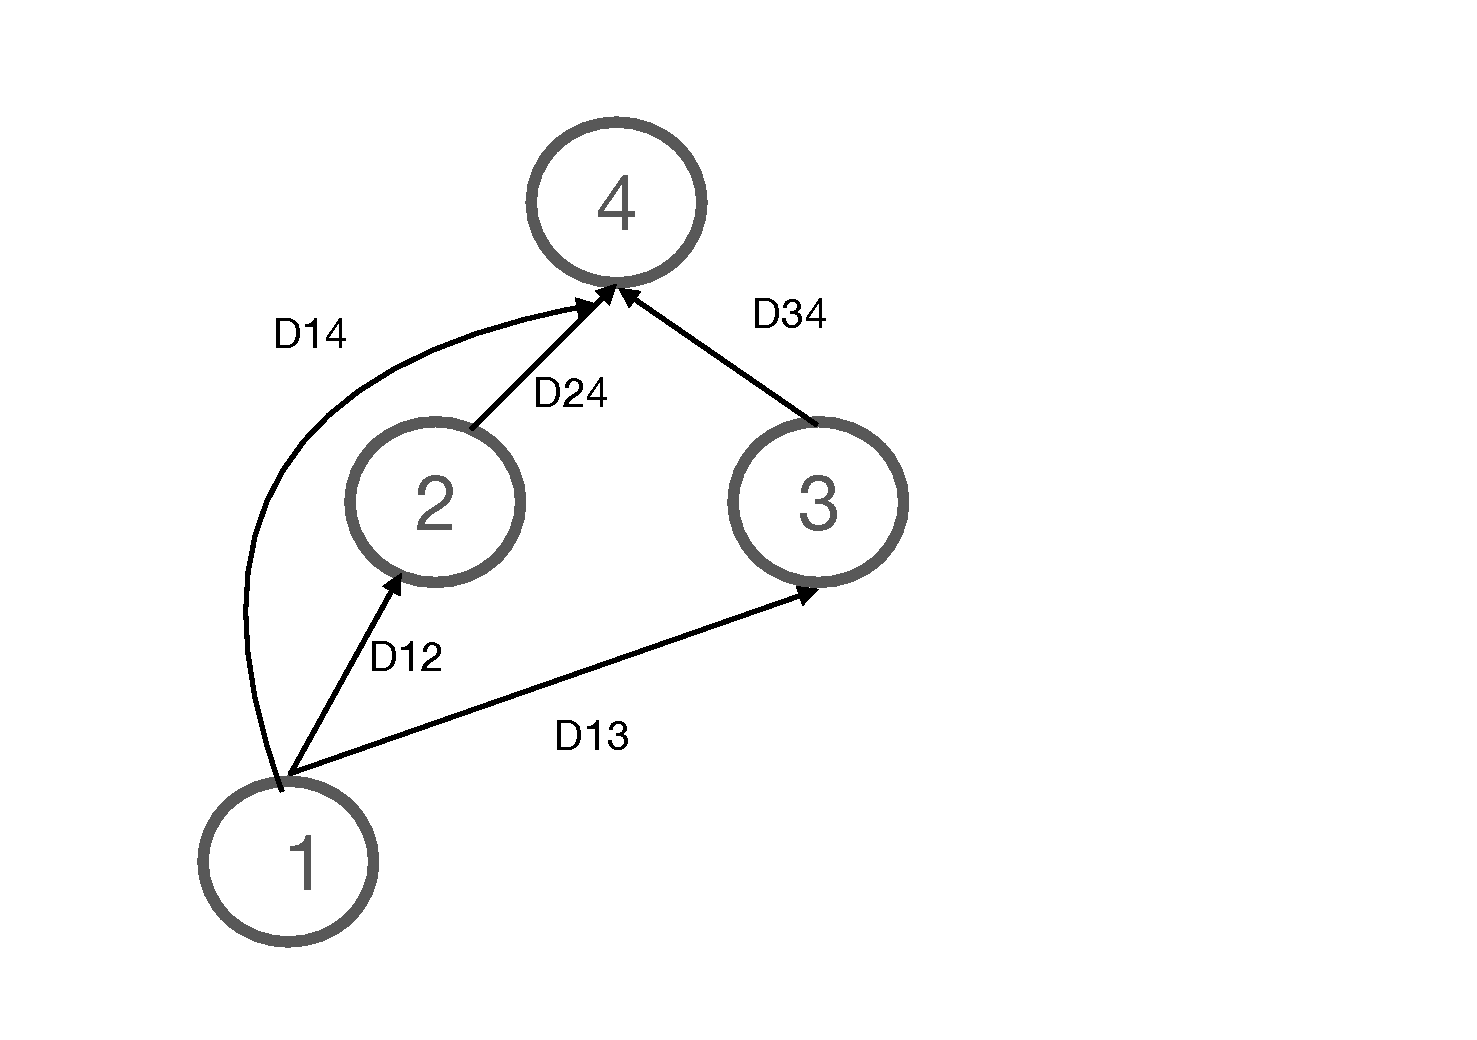
\includegraphics[scale=0.4]{AADImage.pdf}
    \end{figure}
    $$ \frac{d x_4}{d x1} = D14 + D12 * D24 + D13 * D34$$
\end{frame}

\begin{frame}\textbf{XVA計算におけるADのメリット、デメリット}\\
    \begin{itemize}
    \item メリット
    \begin{itemize}
        \item 通常の値の計算の数倍(10未満?)で大量のGreeks計算が可能
        \item 解析的な微分をしているので、差分法のようなバイアスがない
    \end{itemize}
    \item デメリット
    \begin{itemize}
        \item 大量のメモリが必要
        \item On memory で一気通貫で計算しないと厳しい。途中で中間データを出力しながらだと、巨大なヤコビ行列を計算する必要が生じる。 
        \item 途中に滑らかでない関数が入ると一気に依存するポイントのGreeksがおかしくなる
        \item pathごとの微分を行なっていくので、熱核で積分して滑らかになる要素が含まれていない
        $$ E[F(X(t, x))] = (P_t F)(x)$$
    \end{itemize}
    \end{itemize}

\end{frame}

\begin{frame}
    AADの最近の進展
    \begin{itemize}
        \item Treeの縮約技術の進展
        \item Stochastic AAD (Flies) \\
        確率変数のツリーを作る(pathのベクトル)
        \item MVAへの応用
        $$MVA =E[ \sum \phi_{i,j} \frac{\partial V(t)}{\partial X^i(t)} \frac{\partial V(t)}{\partial X^j(t)}]$$
        $$E\left[ \sum \phi_{i,j}  E\left[ \frac{\partial F(X(T))}{\partial X^i(t)} | \mathcal{F}_t\right] E\left[ \frac{\partial F(X(T))}{\partial X^i(t)} | \mathcal{F}_t \right] \right]$$
        \item 条件付期待値の中身
    \end{itemize}
\end{frame}

\begin{frame}
  \textbf{Summary of Greeks calculation of XVA}  
  \begin{itemize}
      \item XVAのGreeksの効率的な計算法として、Freezing法とADの紹介
      \item Freezingは以下の場合はうまくいく
      \begin{itemize}
          \item Markov過程でモデル化された原資産の初期値パラメータに関するGreeks
          \item Implicit法を用いた場合
      \end{itemize}
  \end{itemize}
\end{frame}

\end{document}